\newif\ifvimbug
\vimbugfalse

\ifvimbug
\begin{document}
\fi


\subsection{Approximation in Bernstein-Bézier-Darstellung (4 Punkte)}
\subsubsection{1 Punkt}
\subsubsection{1 Punkt}
\begin{center}
  \makebox[\textwidth]{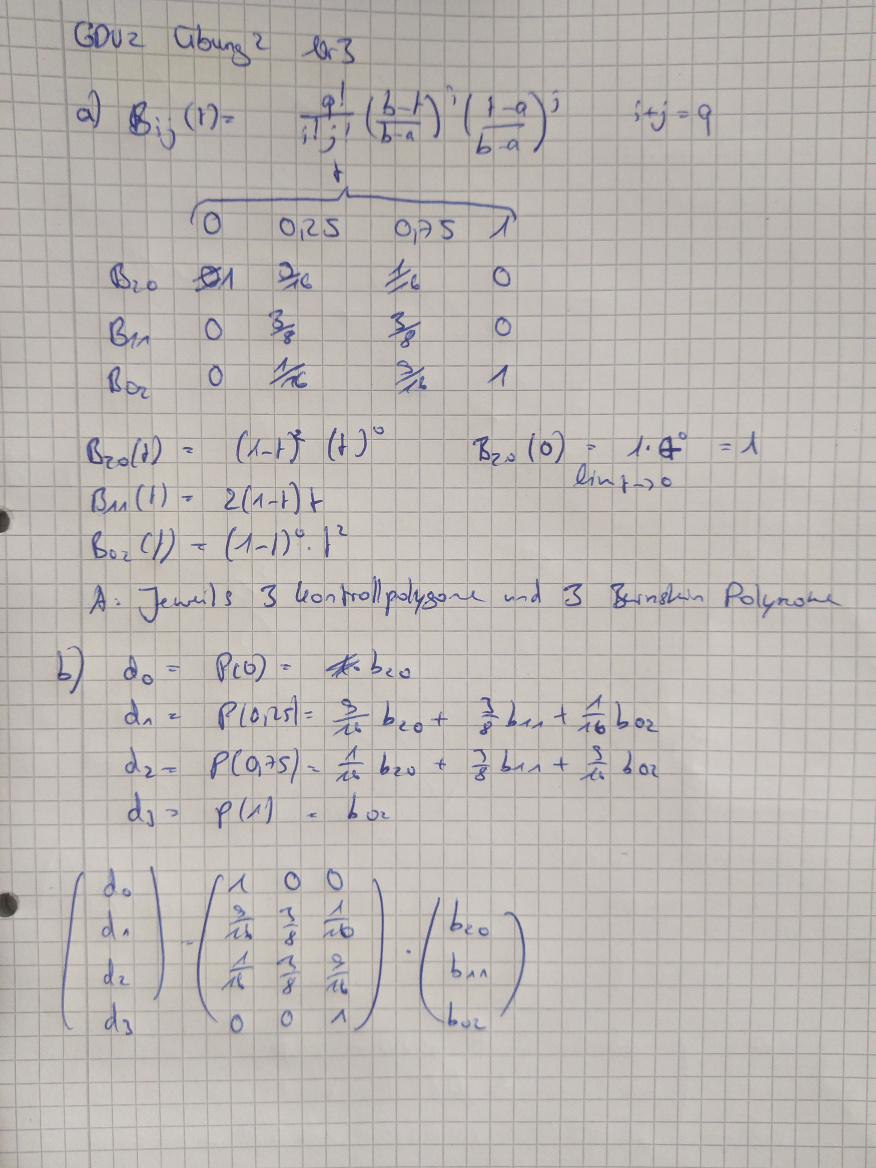
\includegraphics[width=\textwidth]{3ab}}
\end{center}


\subsubsection{1 Punkt}
\begin{center}
  \makebox[\textwidth]{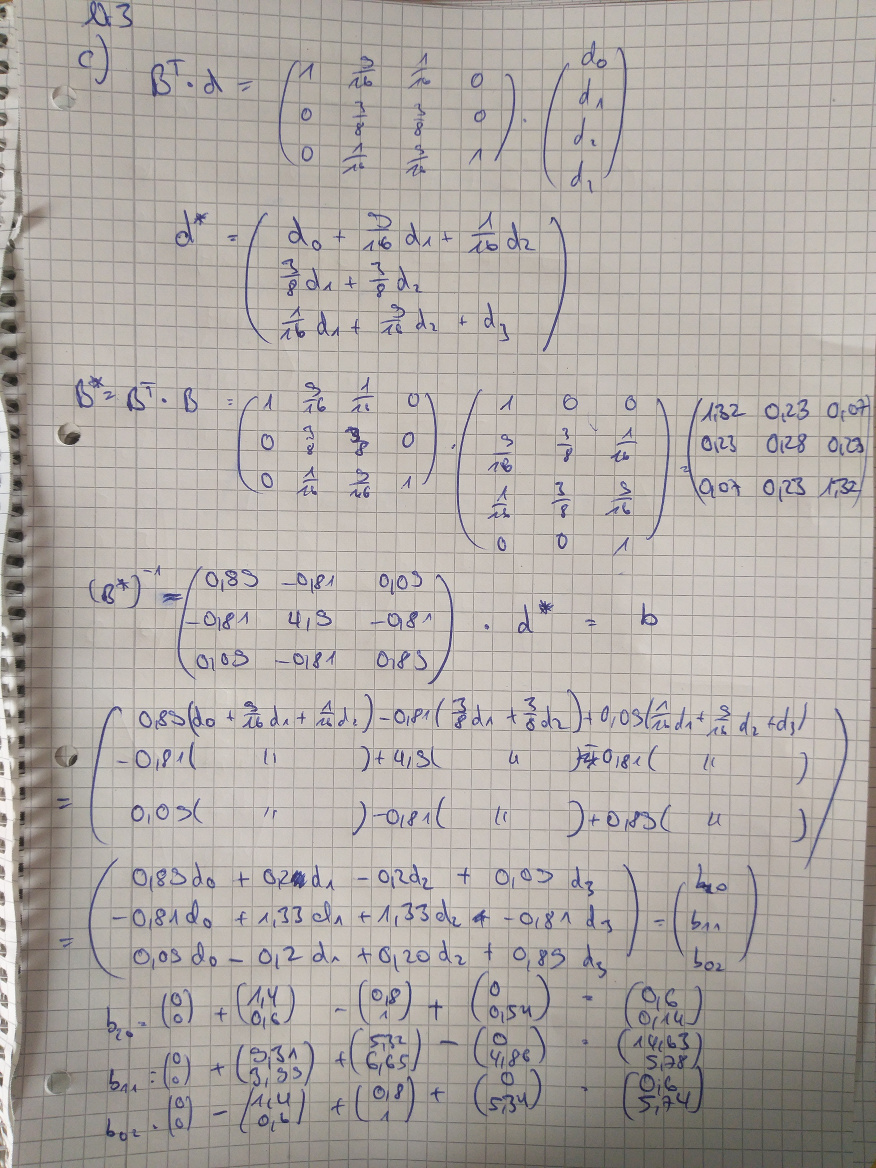
\includegraphics[width=\textwidth]{3c}}
\end{center}
\subsubsection{1 Punkt}
In Rot die Datenpunkte.
In Blau die Kontrollpunkte
und der Verlauf der Approximation in schwarz.\\
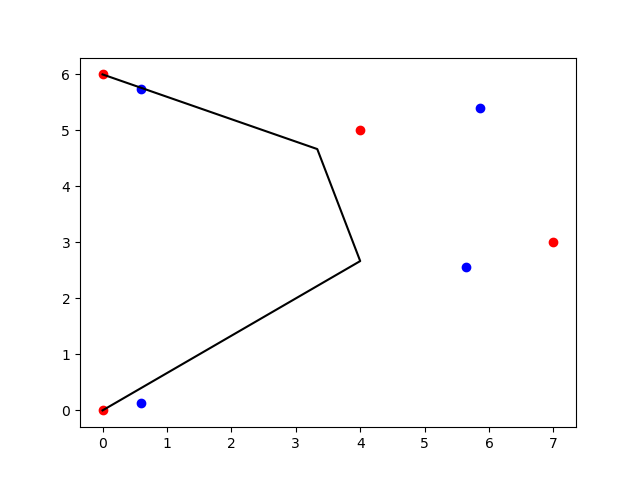
\includegraphics[width=\textwidth]{3d}
